\chapter{- Further technical drawings}
\label{sec:a-techDraw}

\section{Raspberry Pi B+}
\label{sec:goals:rpib}
\begin{figure}[H]
    \centering
    
\includegraphics[angle=90,width=0.75\textwidth]{fig/ch-zz-appendix/A-techDraw/A4_tech_draw_topview_rpi}
    \caption{Technical drawing of Raspberry Pi B+ (topview)}
    \label{fig:parts:rpi_topview}
\end{figure}

\newpage
\section{Adafruit GPS Hat}
\label{sec:goals:gpshat}
\begin{figure}[H]
    \centering
    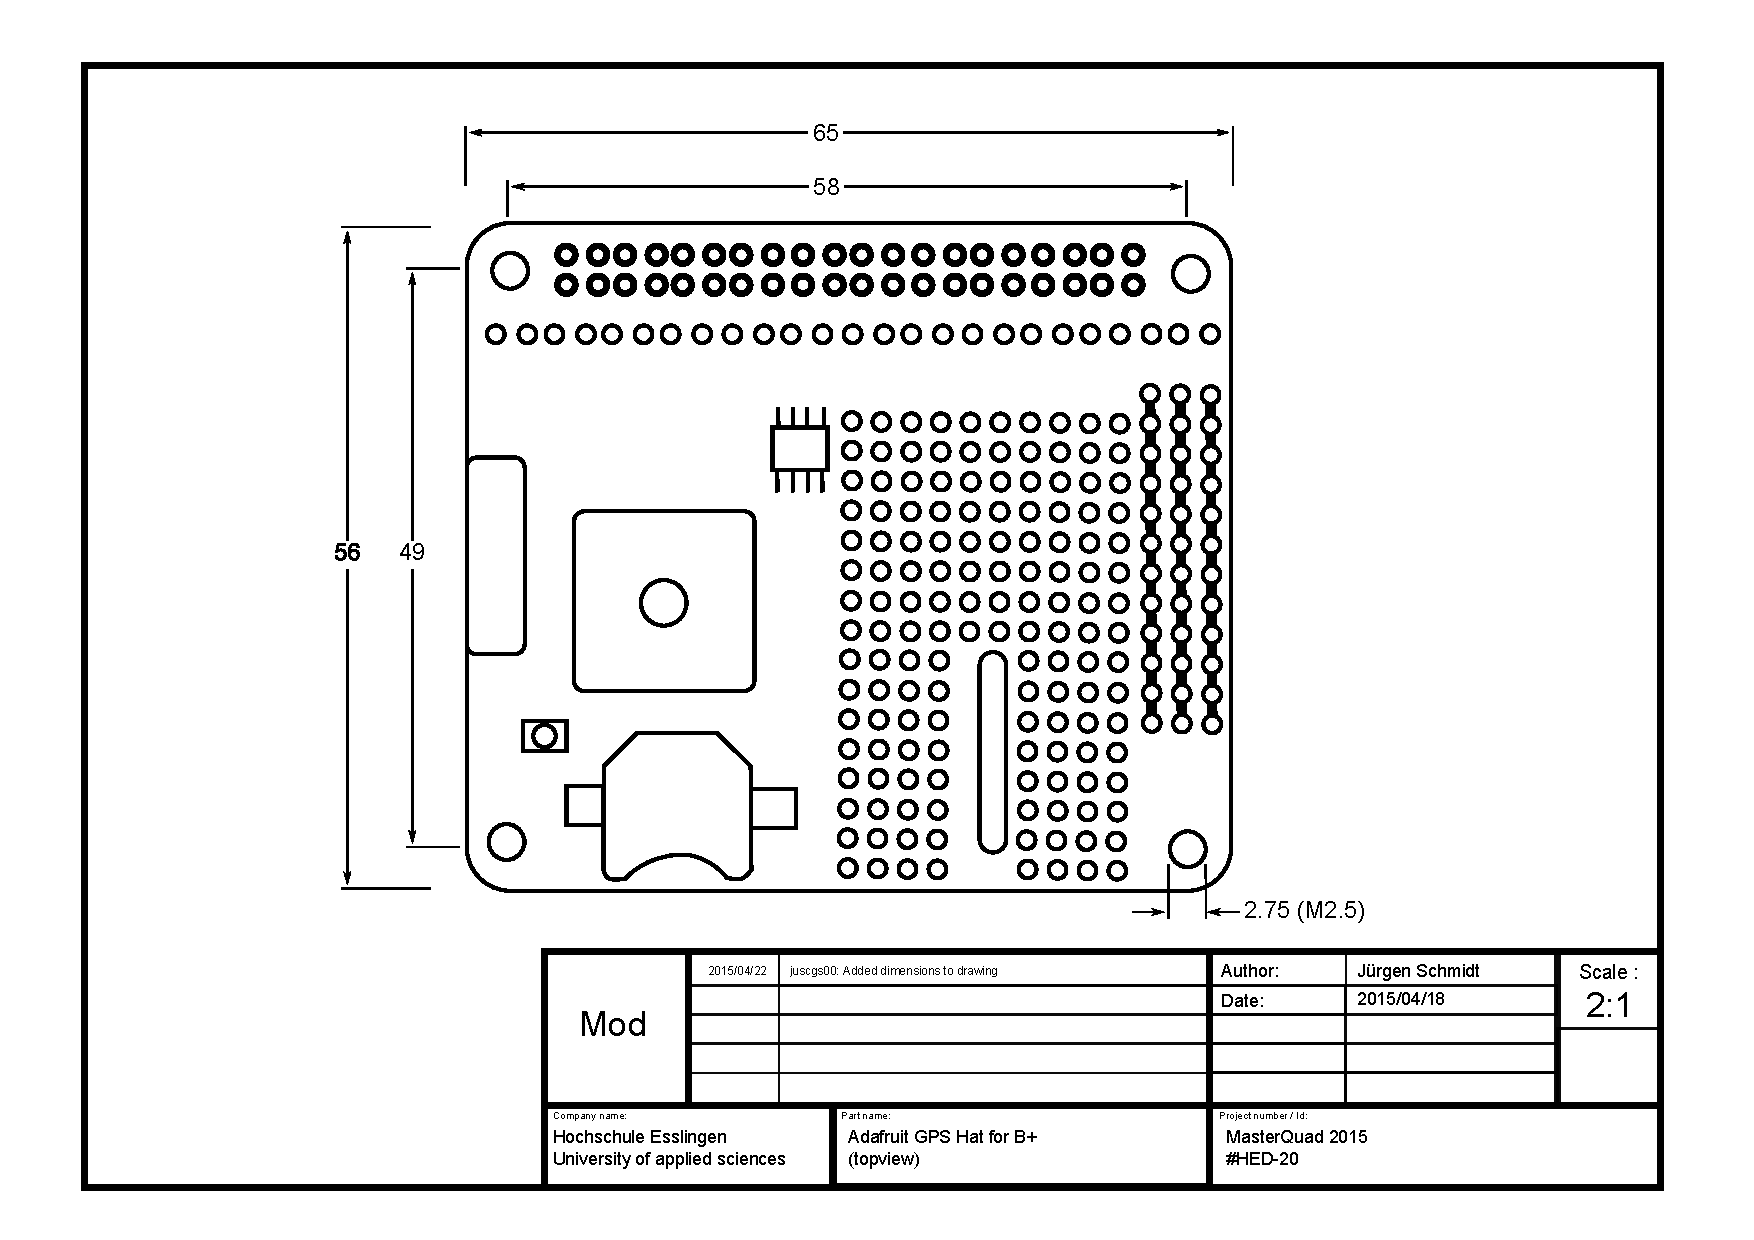
\includegraphics[angle=90,width=0.88\textwidth]{fig/ch-zz-appendix/A-techDraw/A4_tech_draw_topview_gpshat}
    \caption{Technical drawing of Adafruit GPS Hat}
    \label{fig:parts:gps_topview}
\end{figure}

\newpage
\section{Polulu AltIMU v4}
\label{sec:goals:altimu}
\begin{figure}[H]
    \centering
    
\includegraphics[angle=90,width=0.88\textwidth]{fig/ch-zz-appendix/A-techDraw/A4_tech_draw_topview_imu}
    \caption{Technical drawing of Polulu AltIMU v4}
    \label{fig:parts:imu_topview}
\end{figure}

%\newpage
\section{Adafruit 12bit ADC over I2C}
\label{sec:goals:adc}
\begin{figure}[H]
    \centering
    
\includegraphics[angle=90,width=0.88\textwidth]{fig/ch-zz-appendix/A-techDraw/A4_tech_draw_topview_adc}
    \caption{Technical drawing of Adafruit 12bit ADC over I2C}
    \label{fig:parts:adc_topview}
\end{figure}

\chapter{- Code documentation}
\label{sec:b-codeDoc}

For the full code documentation please see Doxygen's HTML output at the SVN repository at
\texttt{/impl/trunk/doc/html/index.html}

The HTML output looks like the following exemplary screen capture in figure \ref{fig:b-codeDoc:doxygenBrowser}.

\begin{figure}[h]
    \centering
    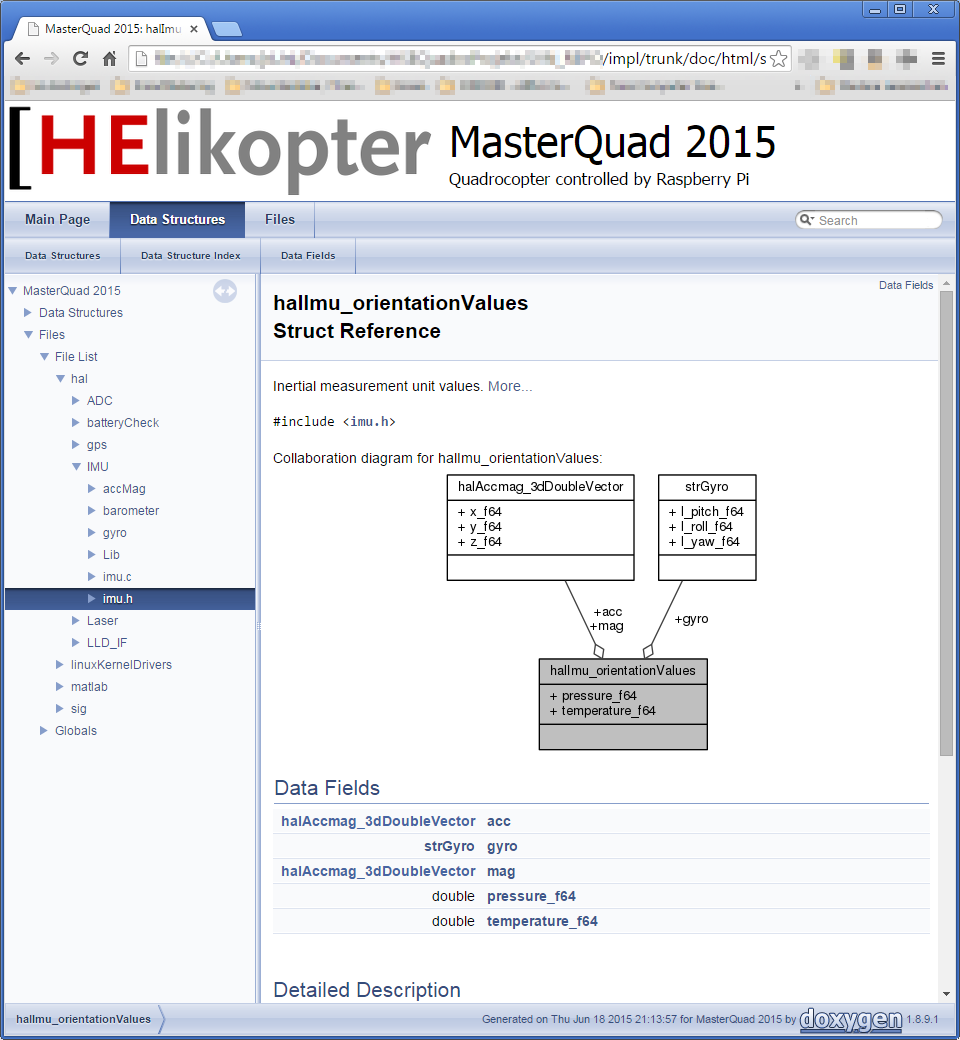
\includegraphics[width=0.86\textwidth]{fig/ch-zz-appendix/B-code-documentation/doxygenHtmlScreen}
    \caption{Screen capture of Doxygen's HTML output for code documentation}
    \label{fig:b-codeDoc:doxygenBrowser}
\end{figure}

\chapter{- Soure code}
\label{sec:append-sourceCode}

\section{S-Function Builder generated C-Code}
\label{sec:c-sFunc-Code}

\subsection{Raw C-Code template of S-Function}
\label{sec:c-sFunc-Code:rawTemplate}
\begin{lstlisting}[caption={[C-Code template 'myUdpSource.c' generated by the S-Function Builder]Complete C-Code template file 'myUdpSource.c' generated by the S-Function Builder according to the example shown in chapter \ref{sec:udpMatlab:simulinkBlock:builder}},label=code:c-sFunc-Code:rawTemplate]
/*
 * File: myUdpSource.c
 *
 *
  *
  *   --- THIS FILE GENERATED BY S-FUNCTION BUILDER: 3.0 ---
  *
  *   This file is an S-function produced by the S-Function
  *   Builder which only recognizes certain fields.  Changes made
  *   outside these fields will be lost the next time the block is
  *   used to load, edit, and resave this file. This file will be overwritten
  *   by the S-function Builder block. If you want to edit this file by hand, 
  *   you must change it only in the area defined as:  
  *
  *        %%%-SFUNWIZ_defines_Changes_BEGIN
  *        #define NAME 'replacement text' 
  *        %%% SFUNWIZ_defines_Changes_END
  *
  *   DO NOT change NAME--Change the 'replacement text' only.
  *
  *   For better compatibility with the Simulink Coder, the
  *   "wrapper" S-function technique is used.  This is discussed
  *   in the Simulink Coder's Manual in the Chapter titled,
  *   "Wrapper S-functions".
  *
  *  -------------------------------------------------------------------------
  * | See matlabroot/simulink/src/sfuntmpl_doc.c for a more detailed template |
  *  ------------------------------------------------------------------------- 
 * Created: Thu Jun 25 20:50:48 2015
 * 
 *
 */

#define S_FUNCTION_LEVEL 2
#define S_FUNCTION_NAME myUdpSource
/*<<<<<<<<<<<<<<<<<<<<<<<<<<<<<<<<<<<<<<<<<<<<<<<<<<<<<<<<<<<<<<<<<*/
/* %%%-SFUNWIZ_defines_Changes_BEGIN --- EDIT HERE TO _END */
#define NUM_INPUTS           0

#define NUM_OUTPUTS          5
/* Output Port  0 */
#define OUT_PORT_0_NAME      acc
#define OUTPUT_0_WIDTH       3
#define OUTPUT_DIMS_0_COL    1
#define OUTPUT_0_DTYPE       real_T
#define OUTPUT_0_COMPLEX     COMPLEX_NO
#define OUT_0_FRAME_BASED    FRAME_NO
#define OUT_0_BUS_BASED      0
#define OUT_0_BUS_NAME       
#define OUT_0_DIMS           1-D
#define OUT_0_ISSIGNED        1
#define OUT_0_WORDLENGTH      8
#define OUT_0_FIXPOINTSCALING 1
#define OUT_0_FRACTIONLENGTH  3
#define OUT_0_BIAS            0
#define OUT_0_SLOPE           0.125
/* Output Port  1 */
#define OUT_PORT_1_NAME      gyro
#define OUTPUT_1_WIDTH       3
#define OUTPUT_DIMS_1_COL    1
#define OUTPUT_1_DTYPE       real_T
#define OUTPUT_1_COMPLEX     COMPLEX_NO
#define OUT_1_FRAME_BASED    FRAME_NO
#define OUT_1_BUS_BASED      0
#define OUT_1_BUS_NAME       
#define OUT_1_DIMS           1-D
#define OUT_1_ISSIGNED        1
#define OUT_1_WORDLENGTH      8
#define OUT_1_FIXPOINTSCALING 1
#define OUT_1_FRACTIONLENGTH  3
#define OUT_1_BIAS            0
#define OUT_1_SLOPE           0.125
/* Output Port  2 */
#define OUT_PORT_2_NAME      mag
#define OUTPUT_2_WIDTH       3
#define OUTPUT_DIMS_2_COL    1
#define OUTPUT_2_DTYPE       real_T
#define OUTPUT_2_COMPLEX     COMPLEX_NO
#define OUT_2_FRAME_BASED    FRAME_NO
#define OUT_2_BUS_BASED      0
#define OUT_2_BUS_NAME       
#define OUT_2_DIMS           1-D
#define OUT_2_ISSIGNED        1
#define OUT_2_WORDLENGTH      8
#define OUT_2_FIXPOINTSCALING 1
#define OUT_2_FRACTIONLENGTH  3
#define OUT_2_BIAS            0
#define OUT_2_SLOPE           0.125
/* Output Port  3 */
#define OUT_PORT_3_NAME      baro
#define OUTPUT_3_WIDTH       1
#define OUTPUT_DIMS_3_COL    1
#define OUTPUT_3_DTYPE       real_T
#define OUTPUT_3_COMPLEX     COMPLEX_NO
#define OUT_3_FRAME_BASED    FRAME_NO
#define OUT_3_BUS_BASED      0
#define OUT_3_BUS_NAME       
#define OUT_3_DIMS           1-D
#define OUT_3_ISSIGNED        1
#define OUT_3_WORDLENGTH      8
#define OUT_3_FIXPOINTSCALING 1
#define OUT_3_FRACTIONLENGTH  3
#define OUT_3_BIAS            0
#define OUT_3_SLOPE           0.125
/* Output Port  4 */
#define OUT_PORT_4_NAME      temp
#define OUTPUT_4_WIDTH       1
#define OUTPUT_DIMS_4_COL    1
#define OUTPUT_4_DTYPE       real_T
#define OUTPUT_4_COMPLEX     COMPLEX_NO
#define OUT_4_FRAME_BASED    FRAME_NO
#define OUT_4_BUS_BASED      0
#define OUT_4_BUS_NAME       
#define OUT_4_DIMS           1-D
#define OUT_4_ISSIGNED        1
#define OUT_4_WORDLENGTH      8
#define OUT_4_FIXPOINTSCALING 1
#define OUT_4_FRACTIONLENGTH  3
#define OUT_4_BIAS            0
#define OUT_4_SLOPE           0.125

#define NPARAMS              1
/* Parameter  1 */
#define PARAMETER_0_NAME      sampleTime
#define PARAMETER_0_DTYPE     real_T
#define PARAMETER_0_COMPLEX   COMPLEX_NO

#define SAMPLE_TIME_0        INHERITED_SAMPLE_TIME
#define NUM_DISC_STATES      0
#define DISC_STATES_IC       [0]
#define NUM_CONT_STATES      0
#define CONT_STATES_IC       [0]

#define SFUNWIZ_GENERATE_TLC 1
#define SOURCEFILES "__SFB__"
#define PANELINDEX           6
#define USE_SIMSTRUCT        0
#define SHOW_COMPILE_STEPS   0                   
#define CREATE_DEBUG_MEXFILE 0
#define SAVE_CODE_ONLY       0
#define SFUNWIZ_REVISION     3.0
/* %%%-SFUNWIZ_defines_Changes_END --- EDIT HERE TO _BEGIN */
/*<<<<<<<<<<<<<<<<<<<<<<<<<<<<<<<<<<<<<<<<<<<<<<<<<<<<<<<<<<<<<<<<<*/
#include "simstruc.h"
#define PARAM_DEF0(S) ssGetSFcnParam(S, 0)

#define IS_PARAM_DOUBLE(pVal) (mxIsNumeric(pVal) && !mxIsLogical(pVal) && !mxIsEmpty(pVal) && !mxIsSparse(pVal) && !mxIsComplex(pVal) && mxIsDouble(pVal))

extern void myUdpSource_Outputs_wrapper(real_T *acc,
																				real_T *gyro,
																				real_T *mag,
																				real_T *baro,
																				real_T *temp, 
																				const real_T  *sampleTime, 
																				const int_T p_width0);

/*====================*
 * S-function methods *
 *====================*/
#define MDL_CHECK_PARAMETERS
 #if defined(MDL_CHECK_PARAMETERS) && defined(MATLAB_MEX_FILE)
   /* Function: mdlCheckParameters =============================================
     * Abstract:
     *    Validate our parameters to verify they are okay.
     */
    static void mdlCheckParameters(SimStruct *S)
    {
     int paramIndex  = 0;
     bool validParam = false;
     /* All parameters must match the S-function Builder Dialog */
     

	 {
	  const mxArray *pVal0 = ssGetSFcnParam(S,0);
	  if (!IS_PARAM_DOUBLE(pVal0)) {
	    validParam = true;
	    paramIndex = 0;
	    goto EXIT_POINT;
	  }
	 }
      
     EXIT_POINT:
      if (validParam) {
          char parameterErrorMsg[1024];
          sprintf(parameterErrorMsg, "The data type and or complexity of parameter  %d does not match the "
                  "information specified in the S-function Builder dialog. "
                  "For non-double parameters you will need to cast them using int8, int16, "
                  "int32, uint8, uint16, uint32 or boolean.", paramIndex + 1);
	  ssSetErrorStatus(S,parameterErrorMsg);
      }
	return;
    }
 #endif /* MDL_CHECK_PARAMETERS */
/* Function: mdlInitializeSizes ===============================================
 * Abstract:
 *   Setup sizes of the various vectors.
 */
static void mdlInitializeSizes(SimStruct *S)
{

    DECL_AND_INIT_DIMSINFO(outputDimsInfo);
    ssSetNumSFcnParams(S, NPARAMS);  /* Number of expected parameters */
      #if defined(MATLAB_MEX_FILE)
	if (ssGetNumSFcnParams(S) == ssGetSFcnParamsCount(S)) {
	  mdlCheckParameters(S);
	  if (ssGetErrorStatus(S) != NULL) {
	    return;
	  }
	 } else {
	   return; /* Parameter mismatch will be reported by Simulink */
	 }
      #endif

    ssSetNumContStates(S, NUM_CONT_STATES);
    ssSetNumDiscStates(S, NUM_DISC_STATES);

    if (!ssSetNumInputPorts(S, NUM_INPUTS)) return;

    if (!ssSetNumOutputPorts(S, NUM_OUTPUTS)) return;
    /* Output Port 0 */
    ssSetOutputPortWidth(S, 0, OUTPUT_0_WIDTH);
    ssSetOutputPortDataType(S, 0, SS_DOUBLE);
    ssSetOutputPortComplexSignal(S, 0, OUTPUT_0_COMPLEX);
    /* Output Port 1 */
    ssSetOutputPortWidth(S, 1, OUTPUT_1_WIDTH);
    ssSetOutputPortDataType(S, 1, SS_DOUBLE);
    ssSetOutputPortComplexSignal(S, 1, OUTPUT_1_COMPLEX);
    /* Output Port 2 */
    ssSetOutputPortWidth(S, 2, OUTPUT_2_WIDTH);
    ssSetOutputPortDataType(S, 2, SS_DOUBLE);
    ssSetOutputPortComplexSignal(S, 2, OUTPUT_2_COMPLEX);
    /* Output Port 3 */
    ssSetOutputPortWidth(S, 3, OUTPUT_3_WIDTH);
    ssSetOutputPortDataType(S, 3, SS_DOUBLE);
    ssSetOutputPortComplexSignal(S, 3, OUTPUT_3_COMPLEX);
    /* Output Port 4 */
    ssSetOutputPortWidth(S, 4, OUTPUT_4_WIDTH);
    ssSetOutputPortDataType(S, 4, SS_DOUBLE);
    ssSetOutputPortComplexSignal(S, 4, OUTPUT_4_COMPLEX);

    ssSetNumSampleTimes(S, 1);
    ssSetNumRWork(S, 0);
    ssSetNumIWork(S, 0);
    ssSetNumPWork(S, 0);
    ssSetNumModes(S, 0);
    ssSetNumNonsampledZCs(S, 0);

    /* Take care when specifying exception free code - see sfuntmpl_doc.c */
    ssSetOptions(S, (SS_OPTION_EXCEPTION_FREE_CODE |
                     SS_OPTION_USE_TLC_WITH_ACCELERATOR | 
		     SS_OPTION_WORKS_WITH_CODE_REUSE));
}

/* Function: mdlInitializeSampleTimes =========================================
 * Abstract:
 *    Specifiy  the sample time.
 */
static void mdlInitializeSampleTimes(SimStruct *S)
{
    ssSetSampleTime(S, 0, SAMPLE_TIME_0);
    ssSetOffsetTime(S, 0, 0.0);
}


#define MDL_START  /* Change to #undef to remove function */
#if defined(MDL_START) 
  /* Function: mdlStart =======================================================
   * Abstract:
   *    This function is called once at start of model execution. If you
   *    have states that should be initialized once, this is the place
   *    to do it.
   */
  static void mdlStart(SimStruct *S)
  {
  }
#endif /*  MDL_START */

#define MDL_SET_OUTPUT_PORT_DATA_TYPE
static void mdlSetOutputPortDataType(SimStruct *S, int port, DTypeId dType)
{
    ssSetOutputPortDataType(S, 0, dType);
}

#define MDL_SET_DEFAULT_PORT_DATA_TYPES
static void mdlSetDefaultPortDataTypes(SimStruct *S)
{
   ssSetOutputPortDataType(S, 0, SS_DOUBLE);
}
/* Function: mdlOutputs =======================================================
 *
*/
static void mdlOutputs(SimStruct *S, int_T tid)
{
    real_T        *acc  = (real_T *)ssGetOutputPortRealSignal(S,0);
    real_T        *gyro  = (real_T *)ssGetOutputPortRealSignal(S,1);
    real_T        *mag  = (real_T *)ssGetOutputPortRealSignal(S,2);
    real_T        *baro  = (real_T *)ssGetOutputPortRealSignal(S,3);
    real_T        *temp  = (real_T *)ssGetOutputPortRealSignal(S,4);
    const int_T   p_width0  = mxGetNumberOfElements(PARAM_DEF0(S));
    const real_T  *sampleTime  = (const real_T *)mxGetData(PARAM_DEF0(S));

    myUdpSource_Outputs_wrapper(acc, gyro, mag, baro, temp, sampleTime, p_width0);
}



/* Function: mdlTerminate =====================================================
 * Abstract:
 *    In this function, you should perform any actions that are necessary
 *    at the termination of a simulation.  For example, if memory was
 *    allocated in mdlStart, this is the place to free it.
 */
static void mdlTerminate(SimStruct *S)
{
}
#ifdef  MATLAB_MEX_FILE    /* Is this file being compiled as a MEX-file? */
#include "simulink.c"      /* MEX-file interface mechanism */
#else
#include "cg_sfun.h"       /* Code generation registration function */
#endif
\end{lstlisting}

\newpage
\subsection{Raw template code of wrapper function}
\label{sec:c-sFunc-Code:wrapperOutputs}

\begin{lstlisting}[caption={[C-Code 'myUdpSource\_wrapper.c' generated by S-Function Builder]Complete C-Code template file 'myUdpSource\_wrapper.c' generated by the S-Function Builder according to the example shown in chapter \ref{sec:udpMatlab:simulinkBlock:builder}},label=code:c-sFunc-Code:rawTemplateWrapper]
/*
  *
  *   --- THIS FILE GENERATED BY S-FUNCTION BUILDER: 3.0 ---
  *
  *   This file is a wrapper S-function produced by the S-Function
  *   Builder which only recognizes certain fields.  Changes made
  *   outside these fields will be lost the next time the block is
  *   used to load, edit, and resave this file. This file will be overwritten
  *   by the S-function Builder block. If you want to edit this file by hand, 
  *   you must change it only in the area defined as:  
  *
  *        %%%-SFUNWIZ_wrapper_XXXXX_Changes_BEGIN 
  *            Your Changes go here
  *        %%%-SFUNWIZ_wrapper_XXXXXX_Changes_END
  *
  *   For better compatibility with the Simulink Coder, the
  *   "wrapper" S-function technique is used.  This is discussed
  *   in the Simulink Coder User's Manual in the Chapter titled,
  *   "Wrapper S-functions".
  *
  *   Created: Sat Jun 27 16:27:07 2015
  */


/*
 * Include Files
 *
 */
#if defined(MATLAB_MEX_FILE)
#include "tmwtypes.h"
#include "simstruc_types.h"
#else
#include "rtwtypes.h"
#endif

/* %%%-SFUNWIZ_wrapper_includes_Changes_BEGIN --- EDIT HERE TO _END */
#include <math.h>
/* %%%-SFUNWIZ_wrapper_includes_Changes_END --- EDIT HERE TO _BEGIN */
#define u_width 
#define y_width 1
/*
 * Create external references here.  
 *
 */
/* %%%-SFUNWIZ_wrapper_externs_Changes_BEGIN --- EDIT HERE TO _END */
/* extern double func(double a); */
/* %%%-SFUNWIZ_wrapper_externs_Changes_END --- EDIT HERE TO _BEGIN */

/*
 * Output functions
 *
 */
void myUdpSource_Outputs_wrapper(real_T *acc,
                          real_T *gyro,
                          real_T *mag,
                          real_T *baro,
                          real_T *temp, 
                           const real_T  *sampleTime, const int_T p_width0)
{
/* %%%-SFUNWIZ_wrapper_Outputs_Changes_BEGIN --- EDIT HERE TO _END */
/* This sample sets the output equal to the input
      y0[0] = u0[0]; 
 For complex signals use: y0[0].re = u0[0].re; 
      y0[0].im = u0[0].im;
      y1[0].re = u1[0].re;
      y1[0].im = u1[0].im;
*/
/* %%%-SFUNWIZ_wrapper_Outputs_Changes_END --- EDIT HERE TO _BEGIN */
}
\end{lstlisting}

\section{MATLAB-Code for Simulink 3D visualization}
\label{sec:d-mFunc-Code}

\begin{lstlisting}[caption={[MATLAB-Code for 3D visualization of orientation angles]MATLAB-Code for a MATLAB-function block to realize a 3D visualization of the Quadrocopter's orientation angles},language=MATLAB,label=code:d-mFunc-Code:3dViz]
function drawBox ( roll, pitch,yaw, objID)
	coder.extrinsic('patch');
	coder.extrinsic('set');

	persistent figureArray patchArray crossArray;

	x1 = [-2 -2 2 2 -2]; 
	y1 = [-4 4 4 -4 -4]; 
	z1 = [0 0 0 0 0 ]; 

	xx = [0 1]; 
	yx = [0 0]; 
	zx = [0 0];

	xy = [0 0]; 
	yy = [0 1]; 
	zy = [0 0];

	xz = [0 0]; 
	yz = [0 0]; 
	zz = [0 1];

	if isempty(figureArray)
			objIDMax=3;
			figureArray=zeros(objIDMax,1);
			figureArray(objID) = figure;
			
			patchArray=zeros(objIDMax,1);
			patchArray(objID) = patch(x1, y1, z1,'r');

			crossArray = zeros(objIDMax,3);
			hold on
			crossArray(objID,1) = plot3(xx,yx,zx,'k','LineWidth',2); %x
			crossArray(objID,2) = plot3(xy,yy,zy,'k','LineWidth',2); %y
			crossArray(objID,3) = plot3(zx,zy,zz,'k','LineWidth',2); %z
					
			xlabel('x'); ylabel('y'); zlabel('z');
			if (objID == 1)
					title('Raw gyro sensors (integrated)');
			else
					title('Filtered (RPi output)');
			end
			grid
			axis([-7 7 -7 7 -7 7])
			view([45 15])
	end

	Rroll = [1,          0,           0;
					 0, cosd(roll), -sind(roll);
					 0, sind(roll), cosd(roll)];
					
	Rpitch = [cosd(pitch), 0, sind(pitch);
					 0,            1,           0;
					 -sind(pitch), 0, cosd(pitch)];
					
	Ryaw = [ cosd(yaw), -sind(yaw),  0;
					 sind(yaw),  cosd(yaw),  0;
					         0,          0,  1];

	xRot=zeros(size(x1));
	yRot=zeros(size(y1));
	zRot=zeros(size(z1));
	for i=1:length(xRot)
			temp=Rroll*Rpitch*Ryaw*[x1(i);y1(i);z1(i)];
			xRot(i)=temp(1);
			yRot(i)=temp(2);
			zRot(i)=temp(3);
	end

	xxRot=zeros(size(xx));
	yxRot=zeros(size(yx));
	zxRot=zeros(size(zx));
	for i=1:length(xxRot)
			temp=Rroll*Rpitch*Ryaw*[xx(i);yx(i);zx(i)];
			xxRot(i)=temp(1);
			yxRot(i)=temp(2);
			zxRot(i)=temp(3);
	end
	set(crossArray( objID,1), 'XData', xxRot);
	set(crossArray( objID,1), 'YData', yxRot);
	set(crossArray( objID,1), 'ZData', zxRot);

	xyRot=zeros(size(xy));
	yyRot=zeros(size(yy));
	zyRot=zeros(size(zy));
	for i=1:length(xyRot)
			temp=Rroll*Rpitch*Ryaw*[xy(i);yy(i);zy(i)];
			xyRot(i)=temp(1);
			yyRot(i)=temp(2);
			zyRot(i)=temp(3);
	end
	set(crossArray( objID,2), 'XData', xyRot);
	set(crossArray( objID,2), 'YData', yyRot);
	set(crossArray( objID,2), 'ZData', zyRot);


	xzRot=zeros(size(xz));
	yzRot=zeros(size(yz));
	zzRot=zeros(size(zz));
	for i=1:length(xzRot)
			temp=Rroll*Rpitch*Ryaw*[xz(i);yz(i);zz(i)];
			xzRot(i)=temp(1);
			yzRot(i)=temp(2);
			zzRot(i)=temp(3);
	end
	set(crossArray( objID,3), 'XData', xzRot);
	set(crossArray( objID,3), 'YData', yzRot);
	set(crossArray( objID,3), 'ZData', zzRot);


	set(patchArray( objID ),'XData', xRot);
	set(patchArray( objID ),'YData', yRot);
	set(patchArray( objID ),'ZData', zRot);
	drawnow
end
\end{lstlisting}

\section{Kernel driver \texttt{ppmDemux}}
\label{sec:append-ppmDemuxCode}

\begin{lstlisting}[caption={[Source code listing of ppmDemux.c]Complete soure code of the proof-of-concept kernel driver \texttt{ppmDemux} to measure the time between to rising edges of GPIO pin 24.},label=code:append-ppmDemuxCode:ppmDemux]
#include <linux/module.h>
#include <linux/fs.h>
#include <linux/cdev.h>
#include <linux/device.h>
#include <linux/gpio.h>
#include <asm/uaccess.h>
#include <linux/interrupt.h>
#include <linux/sched.h>

#include <linux/init.h>
#include <linux/kernel.h>
#include <linux/errno.h>
#include <linux/fs.h>
#include <linux/uaccess.h>
#include <linux/io.h>

#include <asm-generic/errno-base.h>
#include <linux/wait.h>

/*
 * System Timer base address
 *
 * Note: Phys. SoC address 0x7Ennnnnn (as given in data sheet) gets mapped
 *       to 0x20nnnnnn by built-in MMU
 *
 * */
#define TIMER_PAGE_BASE 0x20003000
#define TIMER_OFFSET 	4

#define M_GPIO_NUMBER	24

static dev_t gpio_dev_number;
static struct cdev *driver_object;
static struct class *gpio_class;
static struct device *gpio_dev;
static int rpi_irq_17;
static char *devname = "ppmDemux";
static wait_queue_head_t sleeping_for_ir;

static void *timer_pf;        /* the page frame containing the timer */
static unsigned long *timer_low;
static unsigned long *timer_high;

struct timedInterrupt{
	int 					irqNum;
	unsigned long	timer_l;
	unsigned long	timer_h;
};

static struct timedInterrupt modIrqObj;

static irqreturn_t rpi_gpio_isr( int irq, void *data )
{
	/* wake up read function to retrieve new data */
	wake_up( &sleeping_for_ir );

	return IRQ_HANDLED;
}

static irqreturn_t hard_isr( int irq, void *dev_id )
{
	/* read free running timer (64bit) @ 1MHz */
	modIrqObj.timer_l = readl(timer_low);
	modIrqObj.timer_h = readl(timer_high);

	/* counts rising edges since last read */
	modIrqObj.irqNum += 1;

	return IRQ_WAKE_THREAD;
}

static int config_gpio( int gpionr )
{
	int err, rpi_irq;
	char name[20];

	snprintf( name, sizeof(name), "rpi-gpio-%d", gpionr );
	err = gpio_request( gpionr, name );
	if (err) {
		printk("gpio_request failed %d\n", err);
		return -1;
	}
	err = gpio_direction_input( gpionr );
	if (err) {
		printk("gpio_direction_input failed %d\n", err);
		gpio_free( gpionr );
		return -1;
	}
	rpi_irq = gpio_to_irq( gpionr );
	printk("gpio_to_irq returned %d\n", rpi_irq);
	if (rpi_irq < 0) {
		printk("gpio_to_irq failed %d\n", rpi_irq);
		gpio_free( gpionr );
		return -1;
	}
	err = request_threaded_irq( rpi_irq, hard_isr, rpi_gpio_isr, IRQF_TRIGGER_RISING, devname, driver_object);
	printk("driver_object: %p\n", driver_object);
	if (err) {
		printk("request_irq failed with %d\n", err);
		gpio_free( gpionr );
		return -1;
	}
	printk("gpio %d successfull configured\n", gpionr);
	return rpi_irq;
}

static ssize_t driver_read( struct file *instanz, char __user *user,
		size_t count, loff_t *offset )
{
	unsigned long not_copied, to_copy;

	/* re-init data structure */
	modIrqObj.irqNum 	= 0;
	modIrqObj.timer_l	= 0;
	modIrqObj.timer_h	= 0;

	/* wait for an rising edge event (caught by ISR) */
	wait_event_interruptible( sleeping_for_ir, modIrqObj.irqNum);

	/* copy data to user-sapce */
	to_copy = min( count, sizeof(modIrqObj) );
	not_copied = copy_to_user(user, &(modIrqObj), to_copy);

	return to_copy-not_copied;
}

static struct file_operations fops = {
		.owner= THIS_MODULE,
		.read= driver_read,
};

static int __init mod_init( void )
{
	dev_info(gpio_dev, "mod_init");
	init_waitqueue_head( &sleeping_for_ir );

	if( alloc_chrdev_region(&gpio_dev_number,0,1,"gpioirq24")<0 )
		return -EIO;

	driver_object = cdev_alloc(); /* Anmeldeobjekt reservieren */

	if( driver_object==NULL )
		goto free_device_number;

	driver_object->owner = THIS_MODULE;
	driver_object->ops = &fops;

	if( cdev_add(driver_object,gpio_dev_number,1) )
		goto free_cdev;

	gpio_class = class_create( THIS_MODULE, "gpioirq24" );

	if( IS_ERR( gpio_class ) ) {
		pr_err( "gpioirq17: no udev support\n");
		goto free_cdev;
	}
	gpio_dev = device_create( gpio_class, NULL, gpio_dev_number, NULL, "%s", "gpioirq24" );

	if ( IS_ERR(gpio_dev) )
		goto free_class;

	rpi_irq_17 = config_gpio( M_GPIO_NUMBER );
	if (rpi_irq_17 < 0) {
		goto free_device;
	}

	/* get the mapping for the page frame containing the timer */
	timer_pf = ioremap(TIMER_PAGE_BASE, SZ_4K);
	/* and set the pointer to the timer itself */
	timer_low = (unsigned long*)(timer_pf + TIMER_OFFSET);
	timer_high = (unsigned long*)(timer_pf + TIMER_OFFSET + TIMER_OFFSET);
	pr_info("bcm2708_usec initialized; timer @ %pK\n", timer_low);

	return 0;

	/* ERROR HANDLING (below) */
	free_device:
	device_destroy( gpio_class, gpio_dev_number );
	free_class:
	class_destroy( gpio_class );
	free_cdev:
	kobject_put( &driver_object->kobj );
	free_device_number:
	unregister_chrdev_region( gpio_dev_number, 1 );
	/* if the timer was mapped (final step of successful module init) */
	if (timer_pf)
		/* release the mapping */
		iounmap(timer_pf);
	return -EIO;
}

static void __exit mod_exit( void )
{
	/* if the timer was mapped (final step of successful module init) */
	if (timer_pf)
		/* release the mapping */
		iounmap(timer_pf);

	dev_info(gpio_dev, "mod_exit");
	device_destroy( gpio_class, gpio_dev_number );
	class_destroy( gpio_class );
	cdev_del( driver_object );
	unregister_chrdev_region( gpio_dev_number, 1 );
	free_irq(rpi_irq_17, driver_object);
	gpio_free( M_GPIO_NUMBER );
	return;
}

module_init( mod_init );
module_exit( mod_exit );
MODULE_LICENSE("GPL");
\end{lstlisting}

\begin{lstlisting}[caption={[Source code listing of getPpmDemuxValues.c]Complete soure code of the test file \texttt{getPpmDemuxValues.c} to read the output of the proof-of-concept kernel driver \texttt{ppmDemux}.},label=code:append-ppmDemuxCode:ppmDemusReader]
#include <stdio.h>
#include <fcntl.h>

int main( int argc, char **argv, char **envp )
{
    int fd;

    /* structured data received from kernel driver output */
    struct outputStruct{
        int 					irqNum;
        unsigned long timer_l;
        unsigned long timer_h;
    };

    struct outputStruct localOutputBlock;
    
    unsigned long long newTime = 0;
    unsigned long long oldTime = 0;

    /* open character file handler of kernel driver ppmDemux */    
    fd = open( "/dev/gpioirq24", O_RDONLY );
    if (fd<0) {
        perror("/dev/gpioirq24");
        return -1;
    }

    while (1) {
        unsigned long recvBytes=0;

	/* evaluate only lower part of counter value (wrap around every 
	 * ~4.2 seconds is sufficient for this testing approach) 
	 */
        recvBytes = read( fd, 
													&(localOutputBlock), 
													sizeof(struct outputStruct) );
        newTime = (unsigned long long)localOutputBlock.timer_l; 
        printf("interrupts: %d, delta: %llu us\n",
								localOutputBlock.irqNum, 
								newTime - oldTime );

        oldTime = newTime;
    }
    return 0;
}

\end{lstlisting}

\chapter{- Default login credentials}
\label{sec:d-credentials}

\section{Development Environment}
\label{sec:d-credentials:vm}
\textbf{User:} \texttt{user}\\
\textbf{Password:} \texttt{user}

\section{Raspberry Pi Firmware}
\label{sec:d-credentials:rpi}
\textbf{User:} \texttt{pi}\\
\textbf{Password:} \texttt{raspberry}

\textbf{User:} \texttt{root}\\
\textbf{Password:} \texttt{raspberry}